\begin{enumerate}
	\item What is the number of ordered pairs $\brak{A, B}$ where $A$ and $B$ are subsets of $\{1, 2, \ldots, 5\}$ such that neither $A \subseteq B$ nor $B \subseteq A$?\hfill(PRERMO 2014)
	\item
The Bank of Oslo issues two types of coin: aluminium \brak{denoted \ A} and bronze \brak{denoted \ B}. Marianne has $n$ aluminium coins and $n$ bronze coins, arranged in a row in some arbitrary initial order. A chain is any subsequence of consecutive coins of the same type. Given a fixed positive integer $k$ $\leq$ $2n$, Marianne repeatedly performs the following operation: she identifies the longest chain containing the $k^{th}$  coin from the left, and movees all coins in that chain to the left end of the row. For example, if $n = 4$ and $k = 4$, the process starting from the ordering $AABBBABA$
 would be 
\begin{align}
A A \underline{B} B B A B A \rightarrow B B B \underline{A} A A B A \rightarrow A A \underline{A} B B B B A \rightarrow B B B \underline{B} A A A A \rightarrow .... 
\end{align}
Find all pairs \brak{n,k} with $\brak{1 \leq k \leq 2n }$ such that for every initial ordering, at some moment during the process, the leftmost \brak {n} coins will all be of the same type. 
\hfill(IMO 2022)
\item
Let  $n$ be a positive integer. A Nordic square is an  $n \times n$ board containing all the integers from  $1$ to  $n^{2}$ so that each cell contains exactly one number. Two different cells are considered adjacent if they share a common side. Every cell that is adjacent only to cells containing la
Rger numbers is called a valley. An uphill path is a sequence of one or more cells such that:
\begin{enumerate}
\item
The first cell in the sequence is a valley,
\item
Each subsequent cell in the sequence is adjacent to the previous cell, and
\item
The numbers written in the cells in the sequence are in increasing order.
\end{enumerate}
Find as a function of  $n$, the smallest possible total number of uphill paths in a Nordic square. \hfill(IMO 2022)
\item
Let  $n$  be a positive integer. A $Japanese \ triangle$ consists of  $1 + 2 + \cdots + n$  circles arranged in an equilateral triangular shape such that for each  $i = 1, 2, \ldots, n$  the  $i^{th}$ row contains exactly  $i$  circles, exactly one of which is coloured red. A ninja path in a $Japa
nese \ triangle$ is a sequence of  $n$  circles obtained by starting in the top row, then repeatedly going from a circle to one of the two circles immediately below it and finishing in the bottom row. Here is an example of a $Japanese \ triangle$ with $ n = 6$  along with a $ninja \ path$ in that tr
iangle containing two red circles.
\begin{figure}[h!]
\centering
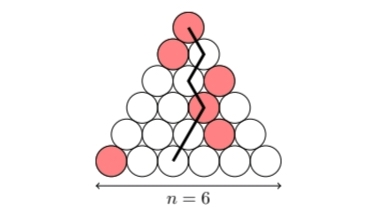
\includegraphics[width=\columnwidth]{figs/img1.jpg}
\caption{Image 1}
\end{figure}
In terms of  $n$, find the greatest $k$ such that in each $Japanese \ triangle$ there is a $ninja \ path$ containing at least  $k$ red circles. \hfill(IMO 2023)
\item
Determine all pairs  $\brak{a, b}$  of positive integers for which there exist positive integers  $g$ and $N$ 
Such that \begin{align}
gcd \brak{a^{n} + b, b + a} = g
\end{align}
Holds for all integers $n \geq N$. Note that $\gcd\brak{x, y}$ denotes the greatest common divisor of integers $x$ and $y$. \hfill(IMO 2024)
\item
Let  $a_{1}, a_{2}, a_{3}, \ldots$  be an infinite sequence of positive integers, and let $N$  be a positive integer. Suppose that, for each  $n \ge N$ ,  $an$ is equal to the number of times  $an$ appears in the list  $a_{1}, a_{2}, \ldots, a_{n-1}$. 
\\ Prove that at least one of the sequences $ a_{1}, a_{3}, a_{5}, \ldots $ and $ a_{2}, a_{4}, a_{6}, \ldots $ is eventually periodic.
		An infinite sequence $b_{1}, b_{2} b_{3}, \ldots$ is eventually periodic if there exist positive integers  $p$  and   $M$ such that  $b_{m+p} = b_{m}$  for all  $m \geq M$ . \hfill(IMO 2024)	
\item
Turbo the snail plays a game on a board with  $2024$ rows and  $2023$  columns. There  are hidden monsters in $2022$ of the cells. Initially, Turbo does not know where any of the monsters   are, but he knows that there Is exactly one monster in each row except the first row and the last  row, and 
That each column contains at most one monster.
Turbo makes a series of attempts to go from the first row to the last row. On each attempt, he chooses   to start on any cell in the first row, then repeatedly moves to an adjacent cell sharing a common Turbo the Tortoise is on a quest to escape from a rectangular grid of cells. Starting on any ce
Ll in the first row, Turbo repeatedly moves to an adjacent cell sharing a common side.\brak{\text{He is allowed to return to a previously }} If he reaches a cell with a monster, his attempt ends and he is transported back to the first row to start a new attempt. The monsters do not move, and Turbo r
emembers whether or not each cell he has visited contains a monster. If he reaches any cell in the last row, his attempt ends and the game is over.
Determine the minimum value of $ n $ for which Turbo has a strategy that guarantees reaching the last row on the  $n^{th}$ attempt or earlier, regardless of the locations of the monsters. \hfill(IMO 2024) 
\item Let
$ S_n = \sum_{k=0}^{n} \frac{1}{\sqrt{k+1} + \sqrt{k}}. $
What is the value of 
$ \sum_{n=1}^{90} \frac{1}{S_n + S_{n-1}}? $\hfill(Prermo 2013)

\item An infinite sequence $x_0, x_1, x_2,.... $of real numbers is said to be bounded if there is a constant $C$ such that $\mydet{x_i} \leq C$ for every $i \geq 0$.
	  Given any real number $a > 1$, construct a bounded infinite sequence $x_0, x_1, x_2,.....$ Such that
	  \begin{align*}\mydet{x_i-x_j}\mydet{i-j}^a \geq 1 \end{align*}
	  for every pair of distinct nonnegative integers $i, j$.\hfill(IMO 1991)
	  \item  Let $n$ be a fixed integer, with $n \geq 2$.$\brak{a}$ Determine the least constant $C$ such that the inequality \begin{align*}\sum_{1\leq i<j\leq n} {x_{i}} {x_{j}} \brak{x_{i}^2 + x_{j}^2} \leq C \brak{\sum_{1\leq i\leq n} x_{i}}^4\end{align*} holds for all real numbers ${x_{1}},....,{x_{n}} \geq 0$. $\brak{b}$ For this constant $C$, determine when equality holds.\hfill(IMO 1999) 

\item  $A$,$ B$, $C$ are positive reals with product$1$. Prove that $\brak{A-1+\frac{1}{B}}\brak{B-1+\frac{1}{C}}\brak{C-1+\frac{1}{A}} \leq 1$.\hfill(IMO 2000)

\item Determine all positive integers relatively prime to all the terms of the infinite sequence
 \begin{align*}
 a_n={2^n}+{3^n}+{6^n},n\geq{1}.
\end{align*} \hfill(IMO 2005)
\item In a mathematical compentition some competitors are friends. Friendship is always mutual. Call a group of competitors a clique if each two of tem are friends.(In particular, any group of fewer than two competitors is a clique.) The number of members of a clique is called its size.                                    Given that, in this competition, the largest size of a clique is even, prove that the competitors can  be arranged in two rooms such that the largest size of  a clique contained in one room is the same as the largest size of a clique contained in the other room.\hfill(IMO 2007)
		\item  Let $n$ and $k$ be positive integers with $k\geq n$ and $k-n$ an even number. Let $2n$ lamps labelled $1, 2,\dots, 2n$ be given, each of which can be either on or off. Initially all the lamps are off.We consider sequences of steps: at each step one of the lamps is switched ( from on to off or from off to on).                                                       Let $N$ be the number of such sequences consisting of $    k$ steps and resulting in the state where lamps $1$ thr    ough $n$ are all on, and lamps $n + 1$ through $2n$ are     all off.                                         Let $M$ be the number of such sequences consisting of $k$ steps, resulting in the state where lamps $1$ through $n$ are all on, and lamps $n + 1$ through $2n$ are all off, but where none of the lamps $n + 1$ through $2n$ is ever switched on.  
		\item Find all functions $f$ : $\brak {0,\infty}$ $\rightarrow$ $\brak{0}$, $\infty$  so, (f is a function from the positive real numbers to the positive real numbers) such that $\frac{(f(w))^2 + (f(x))^2} {f(y)^2 + f(z)^2 }$  for all positive real numbers $w, x, y,z$, satisfying $wx$ = $yz$.\hfill(IMO 2008)
	\item Let $n$ be a positive integer $a_{1},\dots,a_{k}\brak{k\geq 2}$ be distinct integer in the set $\cbrak{1 ,\dots, n}$ such that $n$ divides $a_{i} \brak{a_{i+1}-1}$ for $i=1,\dots, k-1$. Prove that $n$ does not divide $ a_{k} \brak {a_{i}-1}$.\hfill(IMO 2009)
	\item Suppose that $s_{1}, s_{2}, s_{3},\dots $ is a strictly increasing sequence of positive integers such th    at the subsequences       
		\begin{align}
			s_{s1}, s_{s2}, s_{s3},\dots and s_{s1+1}, s_{s2+1}, s_{s3+1},\dots
       \end{align}
are both arithmetic progressions. Prove that the sequence $s_1,s_2,s_3$,...is itself an arithmetic progession.\hfill(IMO 2009) Determine the ratio $\frac{N}{M}$.\hfill(IMO 2008)
\item Find all integers $n\leq3$ for which there exist real numbers \begin{align}01.02.02,\end{align} such that \begin{align} an+1=a1   and  an+2=a2,and \end{align} \begin{align}i=1,2,...,n. aiai+1+1=ai+2 for i=1,2,.....n\end{align}.\hfill (IMO 2018)
\item $A$ site is any point $(x,y)$ in the plane such that $z$ and $y$ are both positive integers less than or equal to $20$.Initially, each of the $400$ sites is unoccupied. Amy and Been take turns placing stones with Amy going first. On her turn, Amy places a new red stone on an unoccupied site such that the distance between any two sites occupied by red stones is not equal to $sqrt(5)$ On his turn, Ben places a new blue stone on any unoccupied site.
	(A site occupied by a blue stone is allowed to be at any distance from any other occupied site.) They stop as soon as a player cannot place a stone. Find the greatest $K$ such that Amy can  ensure that she places at least $K$ red stones, no matter how Ben places his blue stones. \hfill (IMO 2018)
	\item Show that there exists a set $A$ of positive  integers with the following property: For any infinite set {S} of primes there exist two positive integers $m$ $\epsilon$ $A$ and $n \notin A$ each of which is a product of $k$ distinct elements of $S$ for some $k \geq 2$.   \hfill(IMO 1994)
\end{enumerate}

